\hypertarget{abstraction_8c}{
\section{abstraction.c File Reference}
\label{abstraction_8c}\index{abstraction.c@{abstraction.c}}
}
{\tt \#include \char`\"{}abstraction.h\char`\"{}}\par
{\tt \#include \char`\"{}system.h\char`\"{}}\par
{\tt \#include $<$math.h$>$}\par


Include dependency graph for abstraction.c:\nopagebreak
\begin{figure}[H]
\begin{center}
\leavevmode
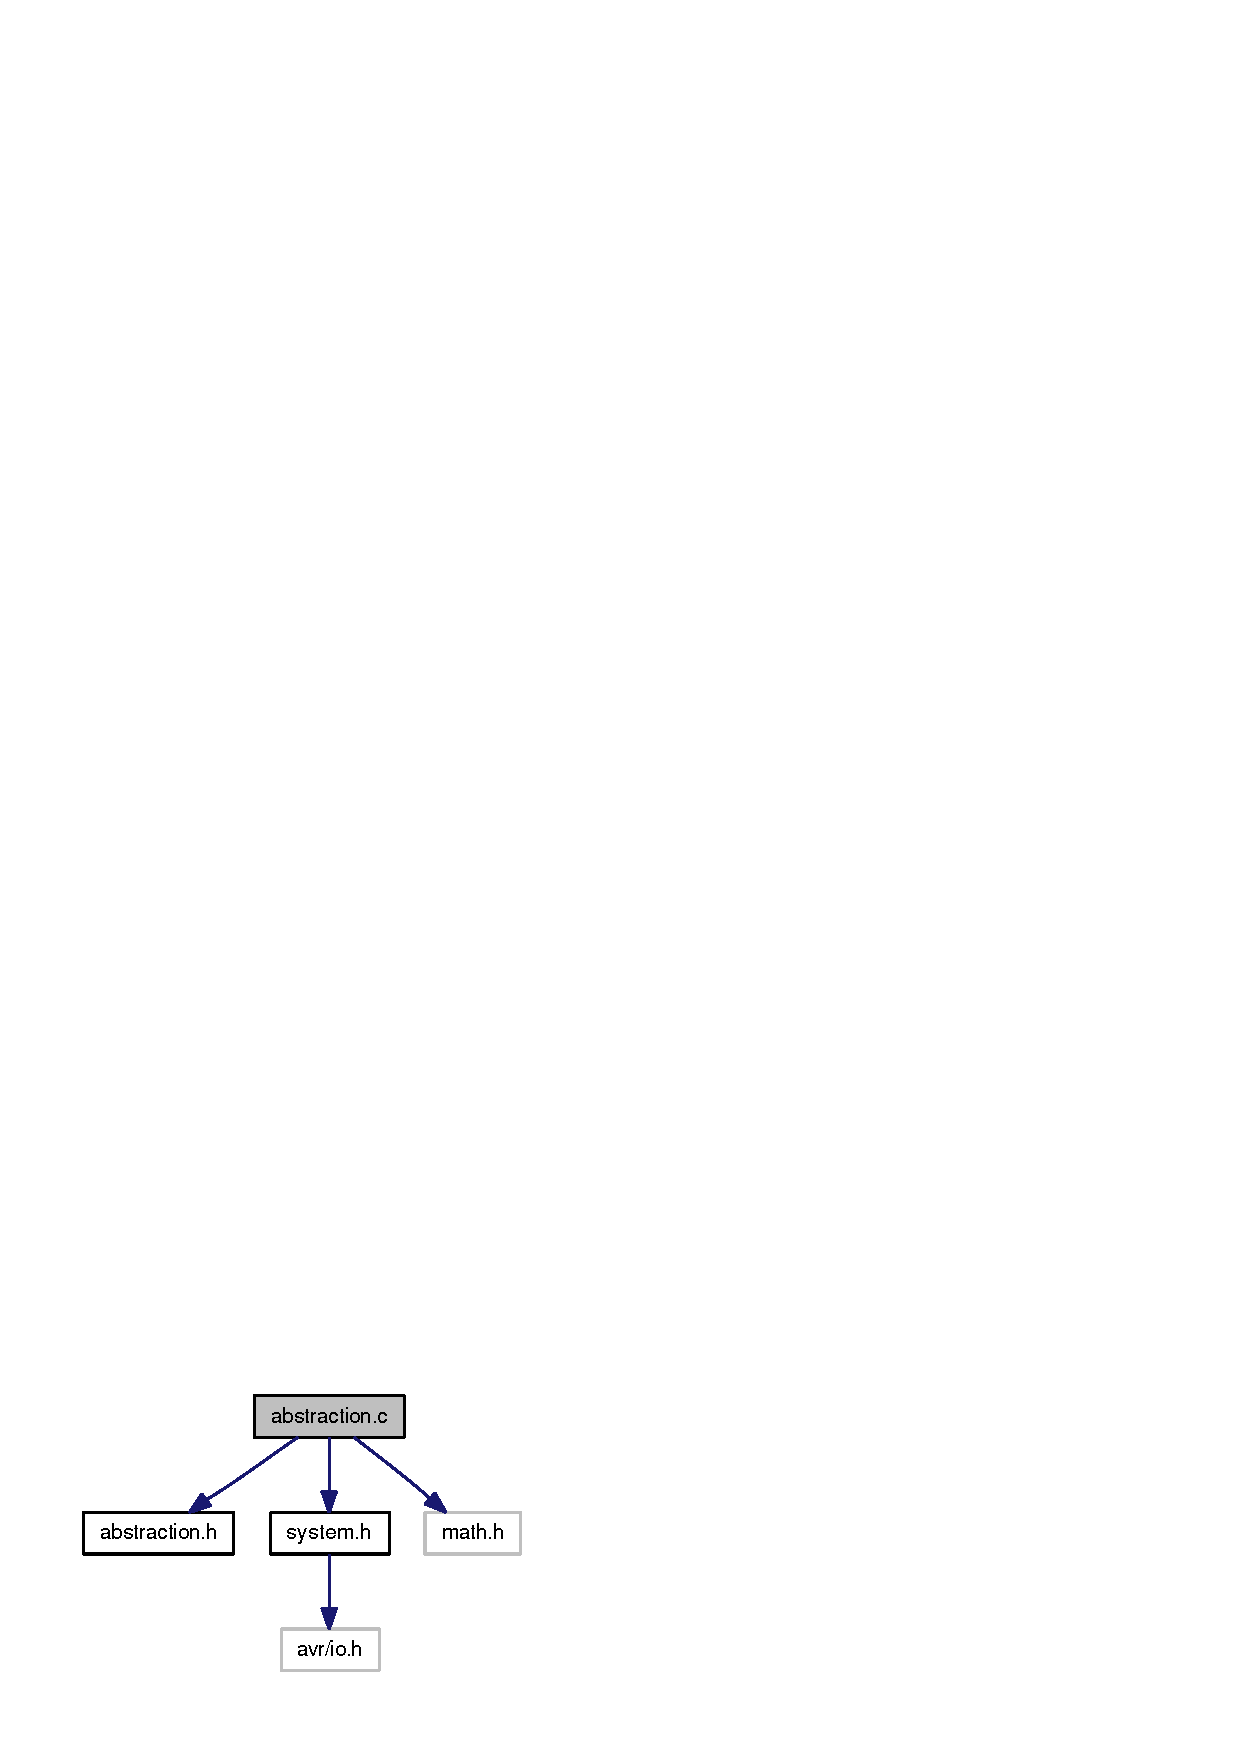
\includegraphics[width=127pt]{abstraction_8c__incl}
\end{center}
\end{figure}
\subsection*{Functions}
\begin{CompactItemize}
\item 
void \hyperlink{abstraction_8c_b45f6a6990e7755a39cc6279e3c09abf}{motor\_\-stuff} ()
\begin{CompactList}\small\item\em Takes controll over the catcher and revolver stepper engines. \item\end{CompactList}\item 
void \hyperlink{abstraction_8c_6a89fa3c3d8ffcbc9f381e23b1d1cb1d}{rotary\_\-encoder\_\-stuff} ()
\begin{CompactList}\small\item\em Takes controll over the rotary encoder (user input) device. \item\end{CompactList}\item 
void \hyperlink{abstraction_8c_acf290466c264ff9b7443af87b69f495}{lightbarrier\_\-stuff} ()
\begin{CompactList}\small\item\em Take control over the lightbarriers. \item\end{CompactList}\item 
void \hyperlink{abstraction_8c_232e74ae3db0daad7e58f233907e3108}{sensor\_\-tcs\_\-stuff} ()
\begin{CompactList}\small\item\em Takes control over the TCS color sensor. \item\end{CompactList}\item 
void \hyperlink{abstraction_8c_7df6f23828e5b8328cf5f5f1d6e06ac2}{vibrator\_\-stuff} ()
\begin{CompactList}\small\item\em Takes control over the shaker (vibrator) device. \item\end{CompactList}\end{CompactItemize}


\subsection{Detailed Description}
All these functions are expected to be called every millisecond by the function ISR (TIMER0\_\-OVF\_\-vect) in the file my\_\-interrupt.c 

Definition in file \hyperlink{abstraction_8c-source}{abstraction.c}.

\subsection{Function Documentation}
\hypertarget{abstraction_8c_acf290466c264ff9b7443af87b69f495}{
\index{abstraction.c@{abstraction.c}!lightbarrier\_\-stuff@{lightbarrier\_\-stuff}}
\index{lightbarrier\_\-stuff@{lightbarrier\_\-stuff}!abstraction.c@{abstraction.c}}
\subsubsection{\setlength{\rightskip}{0pt plus 5cm}void lightbarrier\_\-stuff ()}}
\label{abstraction_8c_acf290466c264ff9b7443af87b69f495}


Take control over the lightbarriers. 

This function is expected to be called regulary. It polls the input pins of the lightbarrier and sets the corresponding flags of lightbarrier struct. This function assumes that lightbarriers are always enabled. 

Definition at line 236 of file abstraction.c.

References IS\_\-LB\_\-CATCHER, IS\_\-LB\_\-REVOLVER, lb\_\-blocked, smartie\_\-sorter\_\-t::lb\_\-catcher, lb\_\-free, smartie\_\-sorter\_\-t::lb\_\-revolver, lightbarrier\_\-t::passes, lightbarrier\_\-t::status, and lightbarrier\_\-t::status\_\-last.

Referenced by ISR().\hypertarget{abstraction_8c_b45f6a6990e7755a39cc6279e3c09abf}{
\index{abstraction.c@{abstraction.c}!motor\_\-stuff@{motor\_\-stuff}}
\index{motor\_\-stuff@{motor\_\-stuff}!abstraction.c@{abstraction.c}}
\subsubsection{\setlength{\rightskip}{0pt plus 5cm}void motor\_\-stuff ()}}
\label{abstraction_8c_b45f6a6990e7755a39cc6279e3c09abf}


Takes controll over the catcher and revolver stepper engines. 

The ramp up is made by linear shrinking the time period t for each step: 

\begin{Code}\begin{verbatim}  Steps
  ^
  |         4t                 3t       2t   t  t  t  t
  *                       *           *     *  *  *  *  *
  |  
  +--+--+--+--+--+--+--+--+--+--+--+--+--+--+--+--+--+--+-> Time
  0  1  2  3  4  5  6  7  8  9 10 11 12 13 14 15 16 17 18
 
 Symbolic diagram, no real values
\end{verbatim}
\end{Code}



This function is expected to be called every millisecond to work properly.

Important setting values are:\begin{itemize}
\item CATCH\_\-STEP\_\-DURATION\item CATCH\_\-RAMP\_\-DURATION\item REV\_\-STEP\_\-DURATION\item REV\_\-RAMP\_\-DURATION \end{itemize}


Definition at line 68 of file abstraction.c.

References smartie\_\-sorter\_\-t::mot\_\-catcher, and smartie\_\-sorter\_\-t::mot\_\-revolver.

Referenced by ISR().\hypertarget{abstraction_8c_6a89fa3c3d8ffcbc9f381e23b1d1cb1d}{
\index{abstraction.c@{abstraction.c}!rotary\_\-encoder\_\-stuff@{rotary\_\-encoder\_\-stuff}}
\index{rotary\_\-encoder\_\-stuff@{rotary\_\-encoder\_\-stuff}!abstraction.c@{abstraction.c}}
\subsubsection{\setlength{\rightskip}{0pt plus 5cm}void rotary\_\-encoder\_\-stuff ()}}
\label{abstraction_8c_6a89fa3c3d8ffcbc9f381e23b1d1cb1d}


Takes controll over the rotary encoder (user input) device. 

This function is expected to be called regulary. It polls the input pins for the rotary encoder and sets the corresponding flags of the rotary\_\-encoder struct. 

Definition at line 170 of file abstraction.c.

References IS\_\-ROTENC\_\-A, IS\_\-ROTENC\_\-AB, IS\_\-ROTENC\_\-B, IS\_\-ROTENC\_\-NONE, IS\_\-ROTENC\_\-PUSH, rotary\_\-encoder\_\-t::left, rotary\_\-encoder\_\-t::push, rotary\_\-encoder\_\-t::pushtmp, rotary\_\-encoder\_\-t::right, smartie\_\-sorter\_\-t::rotenc, ROTENC\_\-A, ROTENC\_\-B, ROTENC\_\-BOTH, ROTENC\_\-NONE, ROTENC\_\-PUSH, and rotary\_\-encoder\_\-t::rottmp.

Referenced by ISR().\hypertarget{abstraction_8c_232e74ae3db0daad7e58f233907e3108}{
\index{abstraction.c@{abstraction.c}!sensor\_\-tcs\_\-stuff@{sensor\_\-tcs\_\-stuff}}
\index{sensor\_\-tcs\_\-stuff@{sensor\_\-tcs\_\-stuff}!abstraction.c@{abstraction.c}}
\subsubsection{\setlength{\rightskip}{0pt plus 5cm}void sensor\_\-tcs\_\-stuff ()}}
\label{abstraction_8c_232e74ae3db0daad7e58f233907e3108}


Takes control over the TCS color sensor. 

This function is expected to be called exectly every millisecond to work properly. This function will read the current color of the smartie.

About the way of color detection please refere to the Main page 

Definition at line 283 of file abstraction.c.

References col\_\-blue, col\_\-green, col\_\-red, COL\_\-SENS\_\-TCS\_\-DISABLE, COL\_\-SENS\_\-TCS\_\-ENABLE, COL\_\-SENS\_\-TCS\_\-FREQ\_\-MESURE\_\-DI, COL\_\-SENS\_\-TCS\_\-FREQ\_\-MESURE\_\-EN, COL\_\-SENS\_\-TCS\_\-SAMPLE\_\-TIME, COL\_\-SENS\_\-TCS\_\-SET\_\-FILTER, col\_\-unknown, color\_\-sensor\_\-tcs\_\-t::color, color\_\-sensor\_\-tcs\_\-t::distance, color\_\-sensor\_\-tcs\_\-t::filter\_\-freq\_\-blue, color\_\-sensor\_\-tcs\_\-t::filter\_\-freq\_\-green, color\_\-sensor\_\-tcs\_\-t::filter\_\-freq\_\-none, color\_\-sensor\_\-tcs\_\-t::filter\_\-freq\_\-red, smartie\_\-sorter\_\-t::sens\_\-tcs, color\_\-sensor\_\-tcs\_\-t::slopes, stat\_\-finished, stat\_\-idle, stat\_\-start\_\-working, stat\_\-stop\_\-working, stat\_\-working, color\_\-sensor\_\-tcs\_\-t::status, color\_\-sensor\_\-tcs\_\-t::status\_\-last, and color\_\-sensor\_\-tcs\_\-t::time.

Referenced by ISR().\hypertarget{abstraction_8c_7df6f23828e5b8328cf5f5f1d6e06ac2}{
\index{abstraction.c@{abstraction.c}!vibrator\_\-stuff@{vibrator\_\-stuff}}
\index{vibrator\_\-stuff@{vibrator\_\-stuff}!abstraction.c@{abstraction.c}}
\subsubsection{\setlength{\rightskip}{0pt plus 5cm}void vibrator\_\-stuff ()}}
\label{abstraction_8c_7df6f23828e5b8328cf5f5f1d6e06ac2}


Takes control over the shaker (vibrator) device. 

This function is expected to be called regulary. It polls the input pins of the shaker and sets the corresponding flags of the shaker struct. This function assumes that 

Definition at line 428 of file abstraction.c.

References vibrator\_\-t::duration, stat\_\-finished, stat\_\-idle, stat\_\-start\_\-working, stat\_\-stop\_\-working, stat\_\-working, vibrator\_\-t::status, vibrator\_\-t::status\_\-last, smartie\_\-sorter\_\-t::vibr, VIBR\_\-DURATION, VIBR\_\-OFF, and VIBR\_\-ON.

Referenced by ISR().